\chapter{Cahier de spécification système}

\section{Introduction}
\label{sec:intro}

La Or-Box est un système destiné aux personnes souffrant de déficience visuelle.
Elle a pour but de les aider au quotidien à reconnaître et distinguer des objets de la vie courante, et ce malgré leur handicap. Quand un objet sera posé sur la Or-Box, celle-ci délivrera à l’utilisateur des messages sonores sur la nature de l’objet.
Dans un premier temps, elle sera limitée à une seule catégorie d’objet (les pièces de monnaie), par la suite nous étendrons ces capacités pour apprendre de nouveaux objets - par exemple des médicaments, des crayons, etc.

\begin{figure}[ht]
  \centerline{
	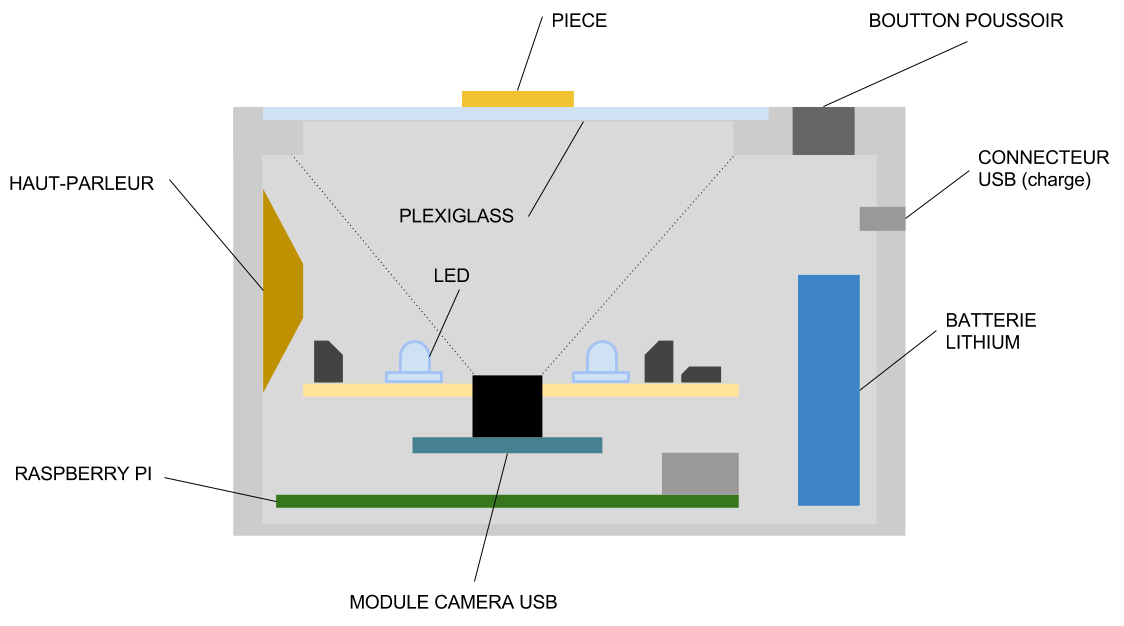
\includegraphics[width=12cm]{img/InitialSketch.png}
  }
  \caption{Croquis du système}
  \label{croquis}
\end{figure}
	
Ce projet a été proposé par Frédéric Rayar.
Il a été initialement mené par un groupe de six étudiants \footnote{Antoine Augay, Valentin Delys, Antoine Fournier, Dylan Lecomte, Jason Loyau, Pierre Robillard} dans le cadre des projets collectifs 2015--2016 de la quatrième année de formation d'informatique industrielle.
Le projet collectif n'ayant pas atteint les objectifs souhaités, j'ai proposé à Frédéric Rayar de le mener à bien en PFE pour l'année 2016-2017.
Le sujet a été accepté comme projet fléché académique.
J'agirai donc comme MOE et M. Rayar comme MOA.

% section intro (end)

\section{Contexte de la réalisation}
 	\subsection{Contexte}
 	\label{sec:contexte}

Malgré les efforts mis sur la notion d'accessibilité, il existe encore de nombreuses barrières qui empêchent les personnes handicapées de vivre de façon indépendante et de participer pleinement à tous les aspects de la vie.
On rappellera notamment que l'Assemblée générale des Nations unies a adopté le 13 décembre 2006 la «Convention relative aux droits des personnes handicapées» qui définit le concept suivant :
\begin{quotation}
	\emph{
	On entend par « conception universelle » la conception de produits, d’équipements, de programmes et de services qui puissent être utilisés par tous, dans toute la mesure possible, sans nécessiter ni adaptation ni conception spéciale.
	La « conception universelle » n’exclut pas les appareils et accessoires fonctionnels pour des catégories particulières de personnes handicapées là où ils sont nécessaires.
	}
\end{quotation}
La Or-Box est donc un de ces appareils qui vise à améliorer l'UX d'objets où la conception universelle n'a pas été appliquée.
Les avancées faites en apprentissage automatique, synthèse vocale et traitement d'images ont rendu ces technologies suffisamment performantes et accessibles pour rendre le projet Or-Box réalisable.
  
  %subsection context (end)
  
	\subsection{Objectifs}
\label{sec:objectifs}
		
Il a été convenu avec la MOA des objectifs suivants :
\begin{itemize}
    \item Un prototype pleinement fonctionnel est attendu à la fin du PFE.
    \item Les contraintes d'industrialisation du produit ne seront pas abordées.
    \item Un taux de reconnaissance de 90\% minimum est attendu sur le cas d'utilisation des pièces de monnaie d'euros.
    \item Les différents jalons académiques devront être respectés.
\end{itemize}

  %subsection objectifs (end)

\section{Description générale}

	\subsection{Environnement du projet}
	\label{sec:envprojet}
	    
Ce projet est la suite directe du projet éponyme mené en DII4A.
La version précédente du projet et ses livrables (prototypes, documentation, code...) sont vus comme une preuve de concept.
Un certain nombre de points ont été validés et seront gardés dans l'état pour ce projet :
\begin{itemize}
	\item Des composants seront récupérés et réutilisés sans modification : la caméra et son objectif, le Raspberry Pi, la batterie, la plaque de verre et le diffuseur.
	\item Des choix technologiques comme celui de la bibliothèque OpenCV --- afin de valoriser la prise de connaissance effectuée.
	\item Certaines parties algorithmiques qui ont été validées : le prétraitement des images (procédure de calibration de la caméra) et la segmentation.
\end{itemize}
				
	%subsection envprojet (end)

	\subsection{Fonctionnalités du système}
\label{sec:foncgales}
	
Le nombre de fonctionnalités offertes par la Or-Box est limité.
Tous les cas d'utilisation doivent rester extrêmement simples du point de vue de l'utilisateur.
Ces différents cas sont illustrés dans la Figure \ref{TopUCD}.

\begin{figure}[!ht]
    \centerline{
	    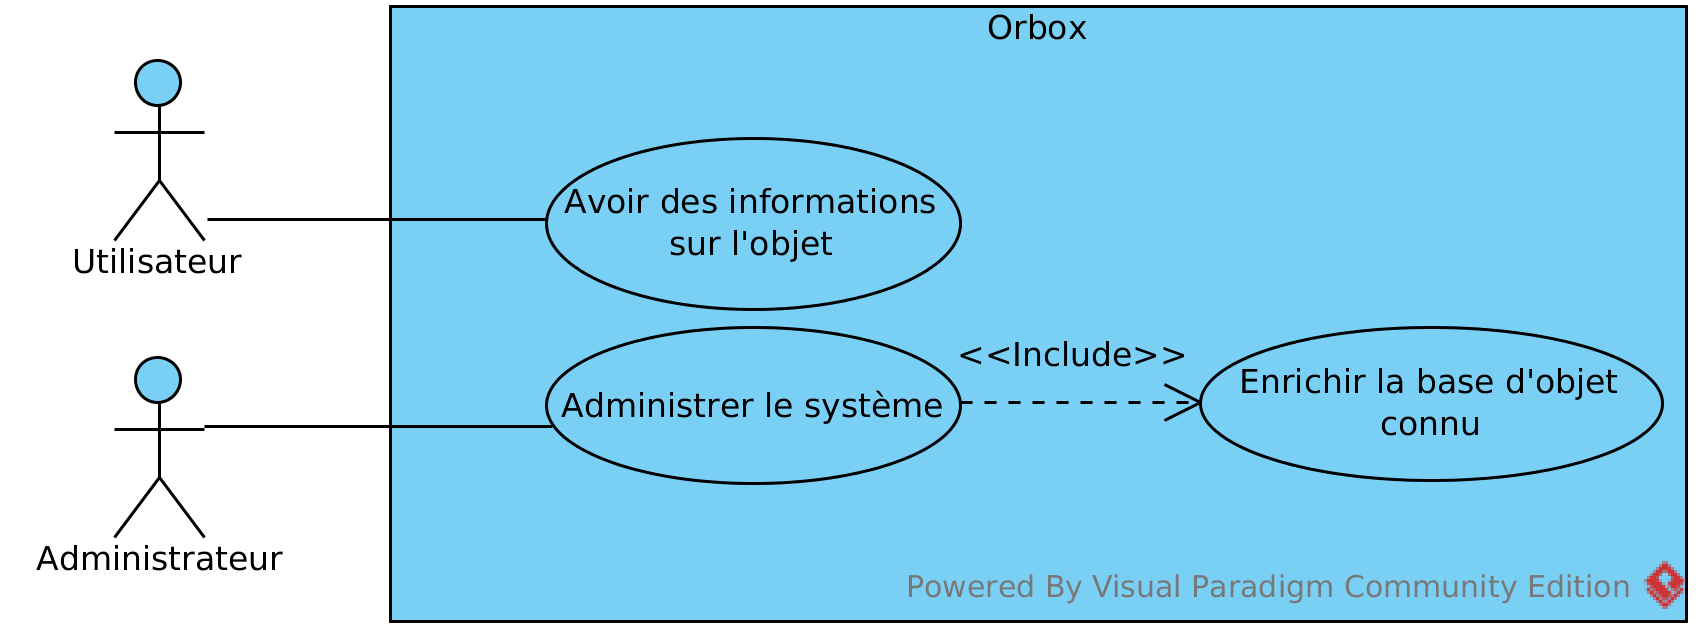
\includegraphics[scale=0.75]{img/SysML_Top_UCD.png}
    }
    \caption{Diagramme des cas d'utilisation}
    \label{TopUCD}
\end{figure}
    
    \subsubsection{Cas d'utilisation : Avoir des informations sur l'objet}
        
Voici le scénario nominal imaginé :
\begin{itemize}
    \item L'utilisateur pose ses pièces sur la plaque de plexiglas
    \item Il fait une requête avec un appui court sur le bouton poussoir.
    \item Les LED de la Or-Box s'allument et une première image est capturée.
    \item Les LED s’éteignent et une deuxième image est capturée.
    \item Après analyse des deux images, la Or-Box fait une annonce vocale --- soit de la somme totale des pièces, soit une énumération des objets reconnus.
\end{itemize}
            
    \subsubsection{Cas d'utilisation : Administrer le système}

Administrer le système consiste à :
\begin{itemize}
    \item Régler la langue pour la description audio.
    \item Choisir les algorithmes et les data sets utilisés.
    \item Changer les messages audio associés à chaque objet.
    \item Faire des opérations (CRUD) sur les objets.
\end{itemize}

Mais aussi pouvoir enrichir la base d'objet connu, c'est-à-dire :
\begin{itemize}
    \item Prendre une paire de photos avec la Or-Box (éclairé \& non éclairé) et effectuer la segmentation.
    \item Renseigner pour chaque segment trouvé la classe (l'objet) qu'il contient.
\end{itemize}


	\subsection{Caractéristiques des utilisateurs}
	\label{sec:caracUser}

Ils existent deux types d'acteurs qui interagissent avec la Or-Box (voir Figure \ref{TopUCD}).

Les premiers sont les utilisateurs, ils sont la raison pour le cas d'utilisation "Avoir des informations sur l'objet".
Ce sont des personnes souffrant de déficience visuelle --- l'interface entre l'utilisateur et la Or-Box doit tenir compte de cette particularité.
On ne fait pas de supposition sur leur niveau de handicap.

Les deuxièmes sont les administrateurs.
Ils n'ont pas de connaissance particulière de l'informatique ni une connaissance préalable de l'application.
L'administrateur devra donc être guidé dans sa tâche (via un manuel d'utilisation simple et lisible et/ou un tutoriel intégré).

%Identifier les différents types d'utilisateurs du système. Pour chacun on devra préciser les caractéristiques qui affecteront l'interface utilisateur (menus, commandes textuelles,\ldots) :
%\begin{itemize}
%	\item connaissance ou non de l'informatique~;
%	\item expérience de l'application~;
%	\item utilisateurs réguliers et/ou occasionnels~;
%	\item droits d'accès utilisateurs.
%\end{itemize}

\subsection{Contraintes de développement, d'exploitation et de maintenance}
\label{Contraintes}

Les contraintes qui s'appliquent sur la Or-Box ont été formaliser sous la forme de trois diagrammes d'exigences SysML --- Figure \ref{RDNominal}, \ref{RDEmbedded} \& \ref{RDProject} respectivement page \pageref{RDNominal}, \pageref{RDEmbedded} \& \pageref{RDProject}.
Pour chaque contrainte est spécifié :
\begin{description}
    \item[Le type] parmi "fonctionnelle", "performance" et "interface"
    \item[La méthode de vérification] parmi "Analyse", "Démonstration", "Inspection" et "Test"
    \item[Le statut] parmi "Approuvé", "Obligatoire" et "Proposé"
\end{description}

\begin{figure}[H]
    \centering
    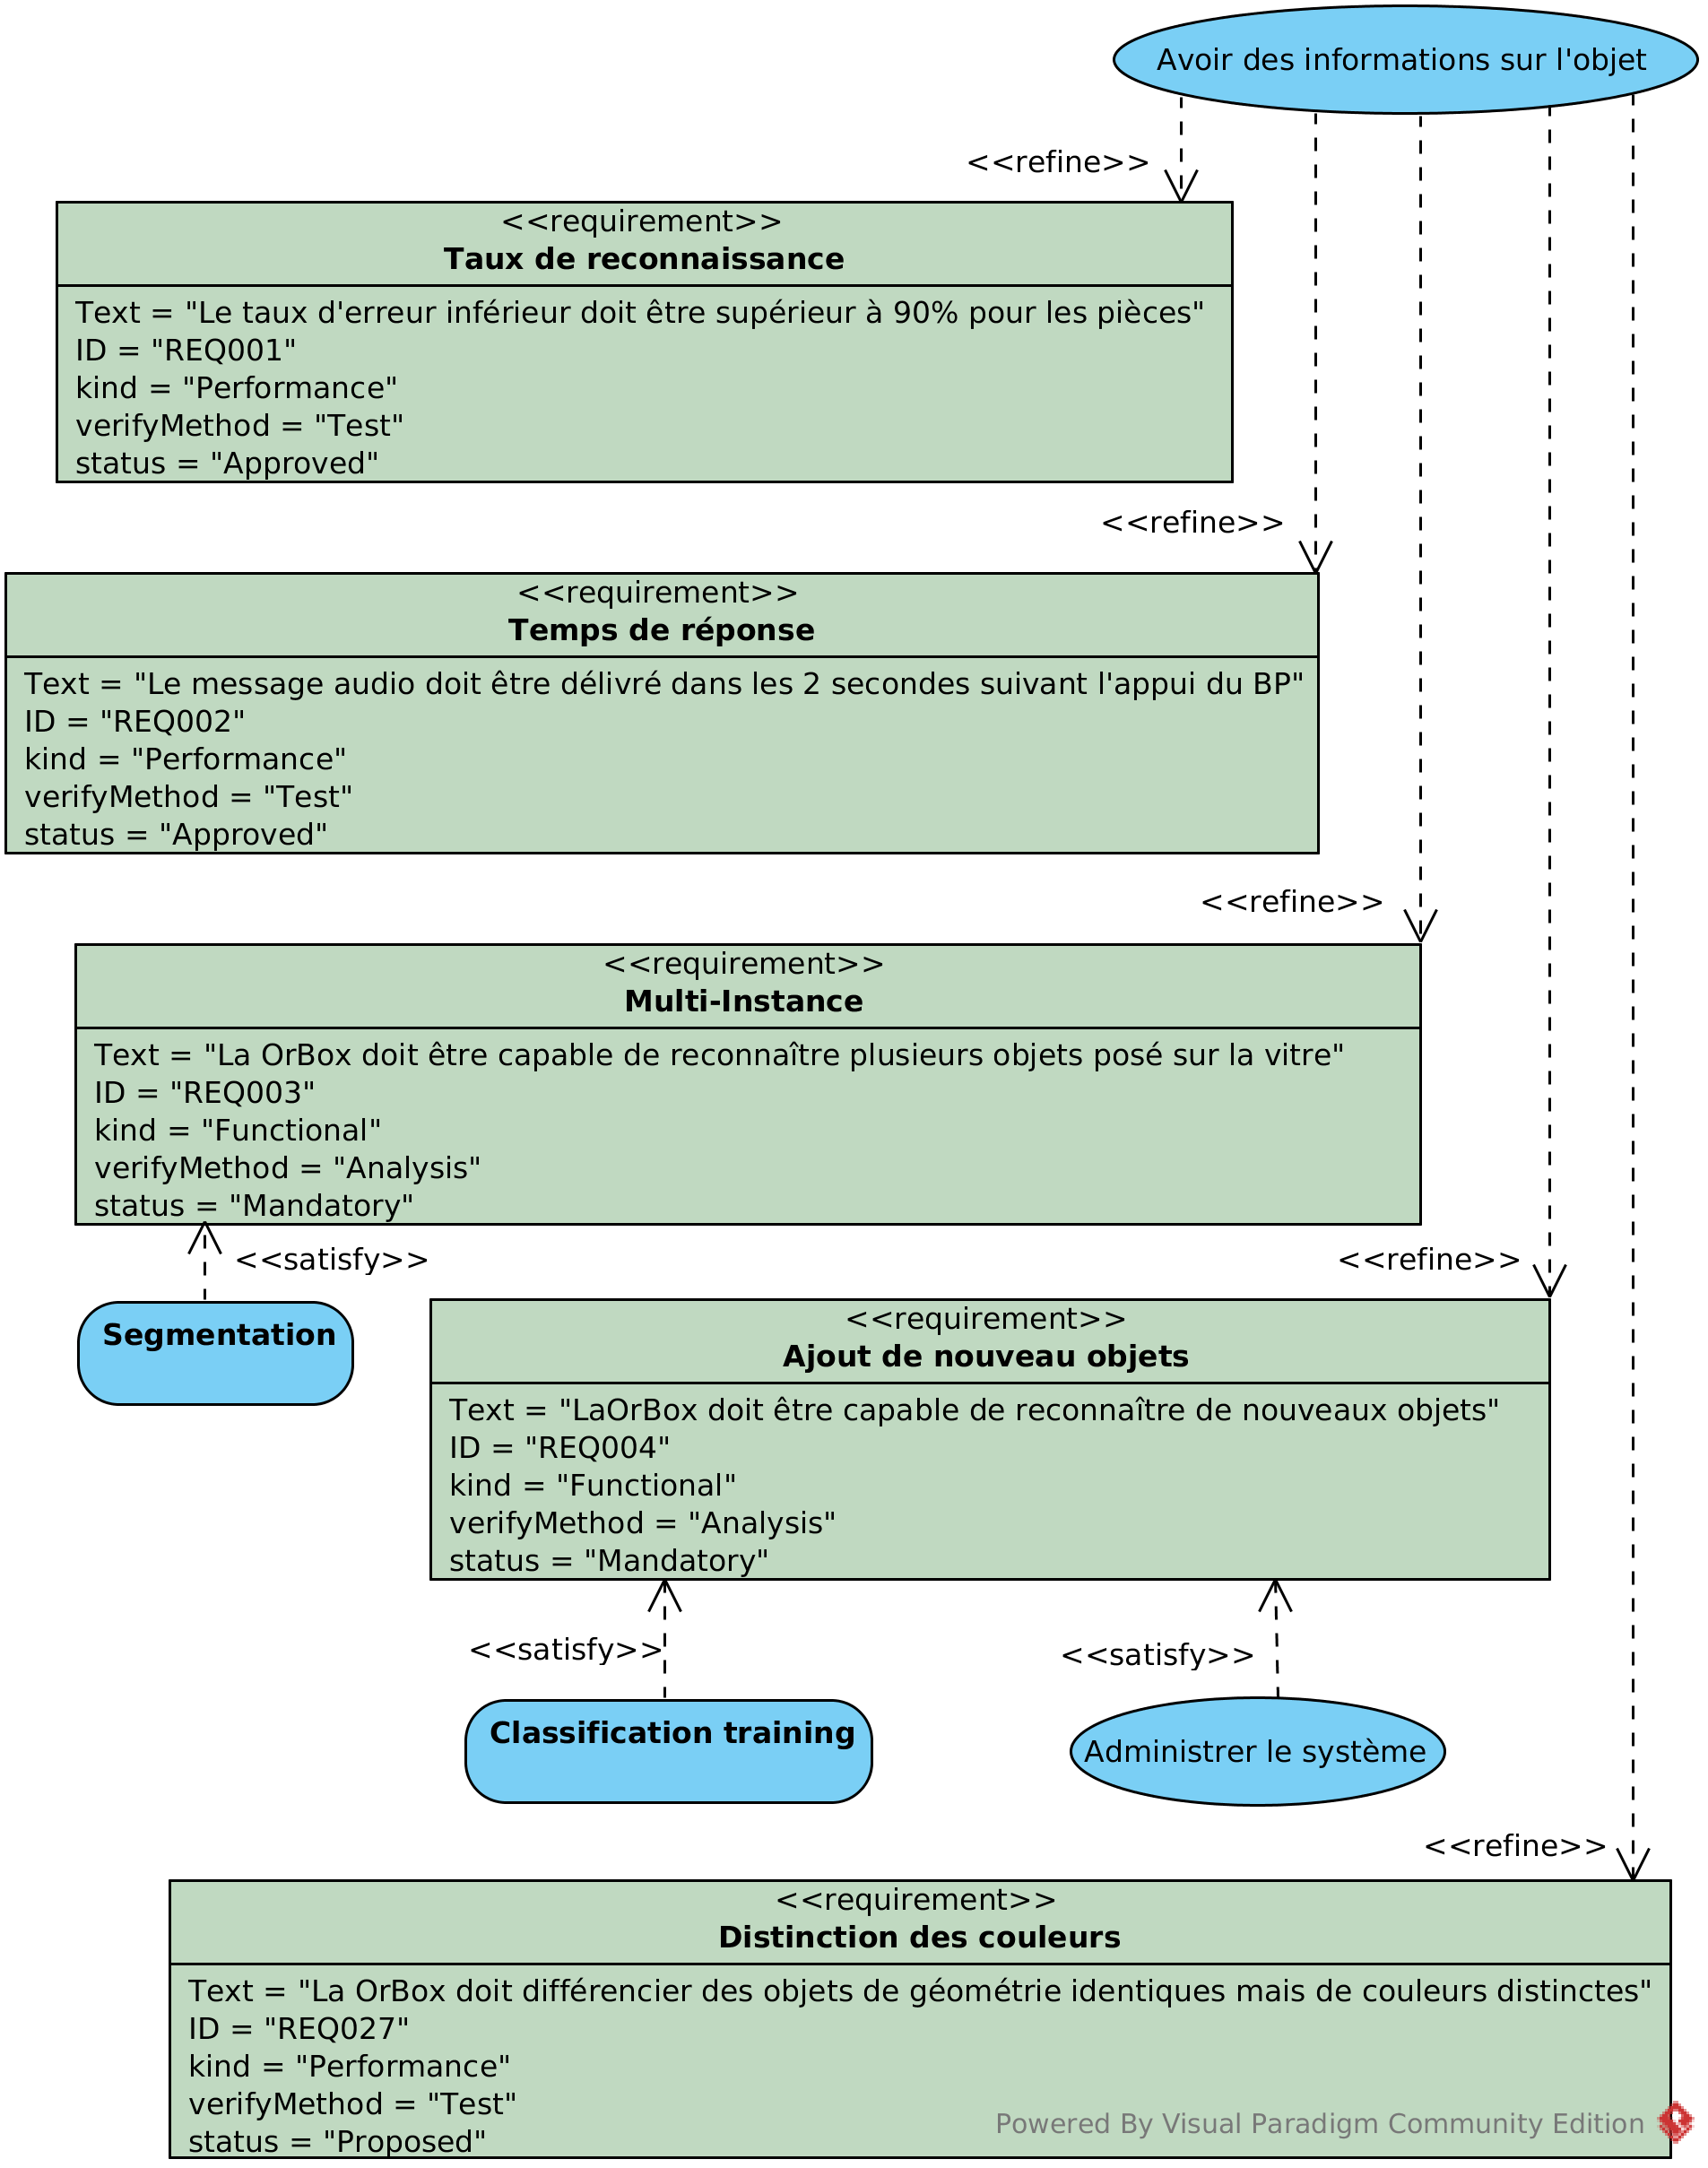
\includegraphics[scale=0.75]{img/SysML_Nominal_RD.png}
    \caption{Diagramme des exigences affinant "Avoir des informations sur l'objet"}
    \label{RDNominal}
\end{figure}

\begin{figure}[H]
    \centering
    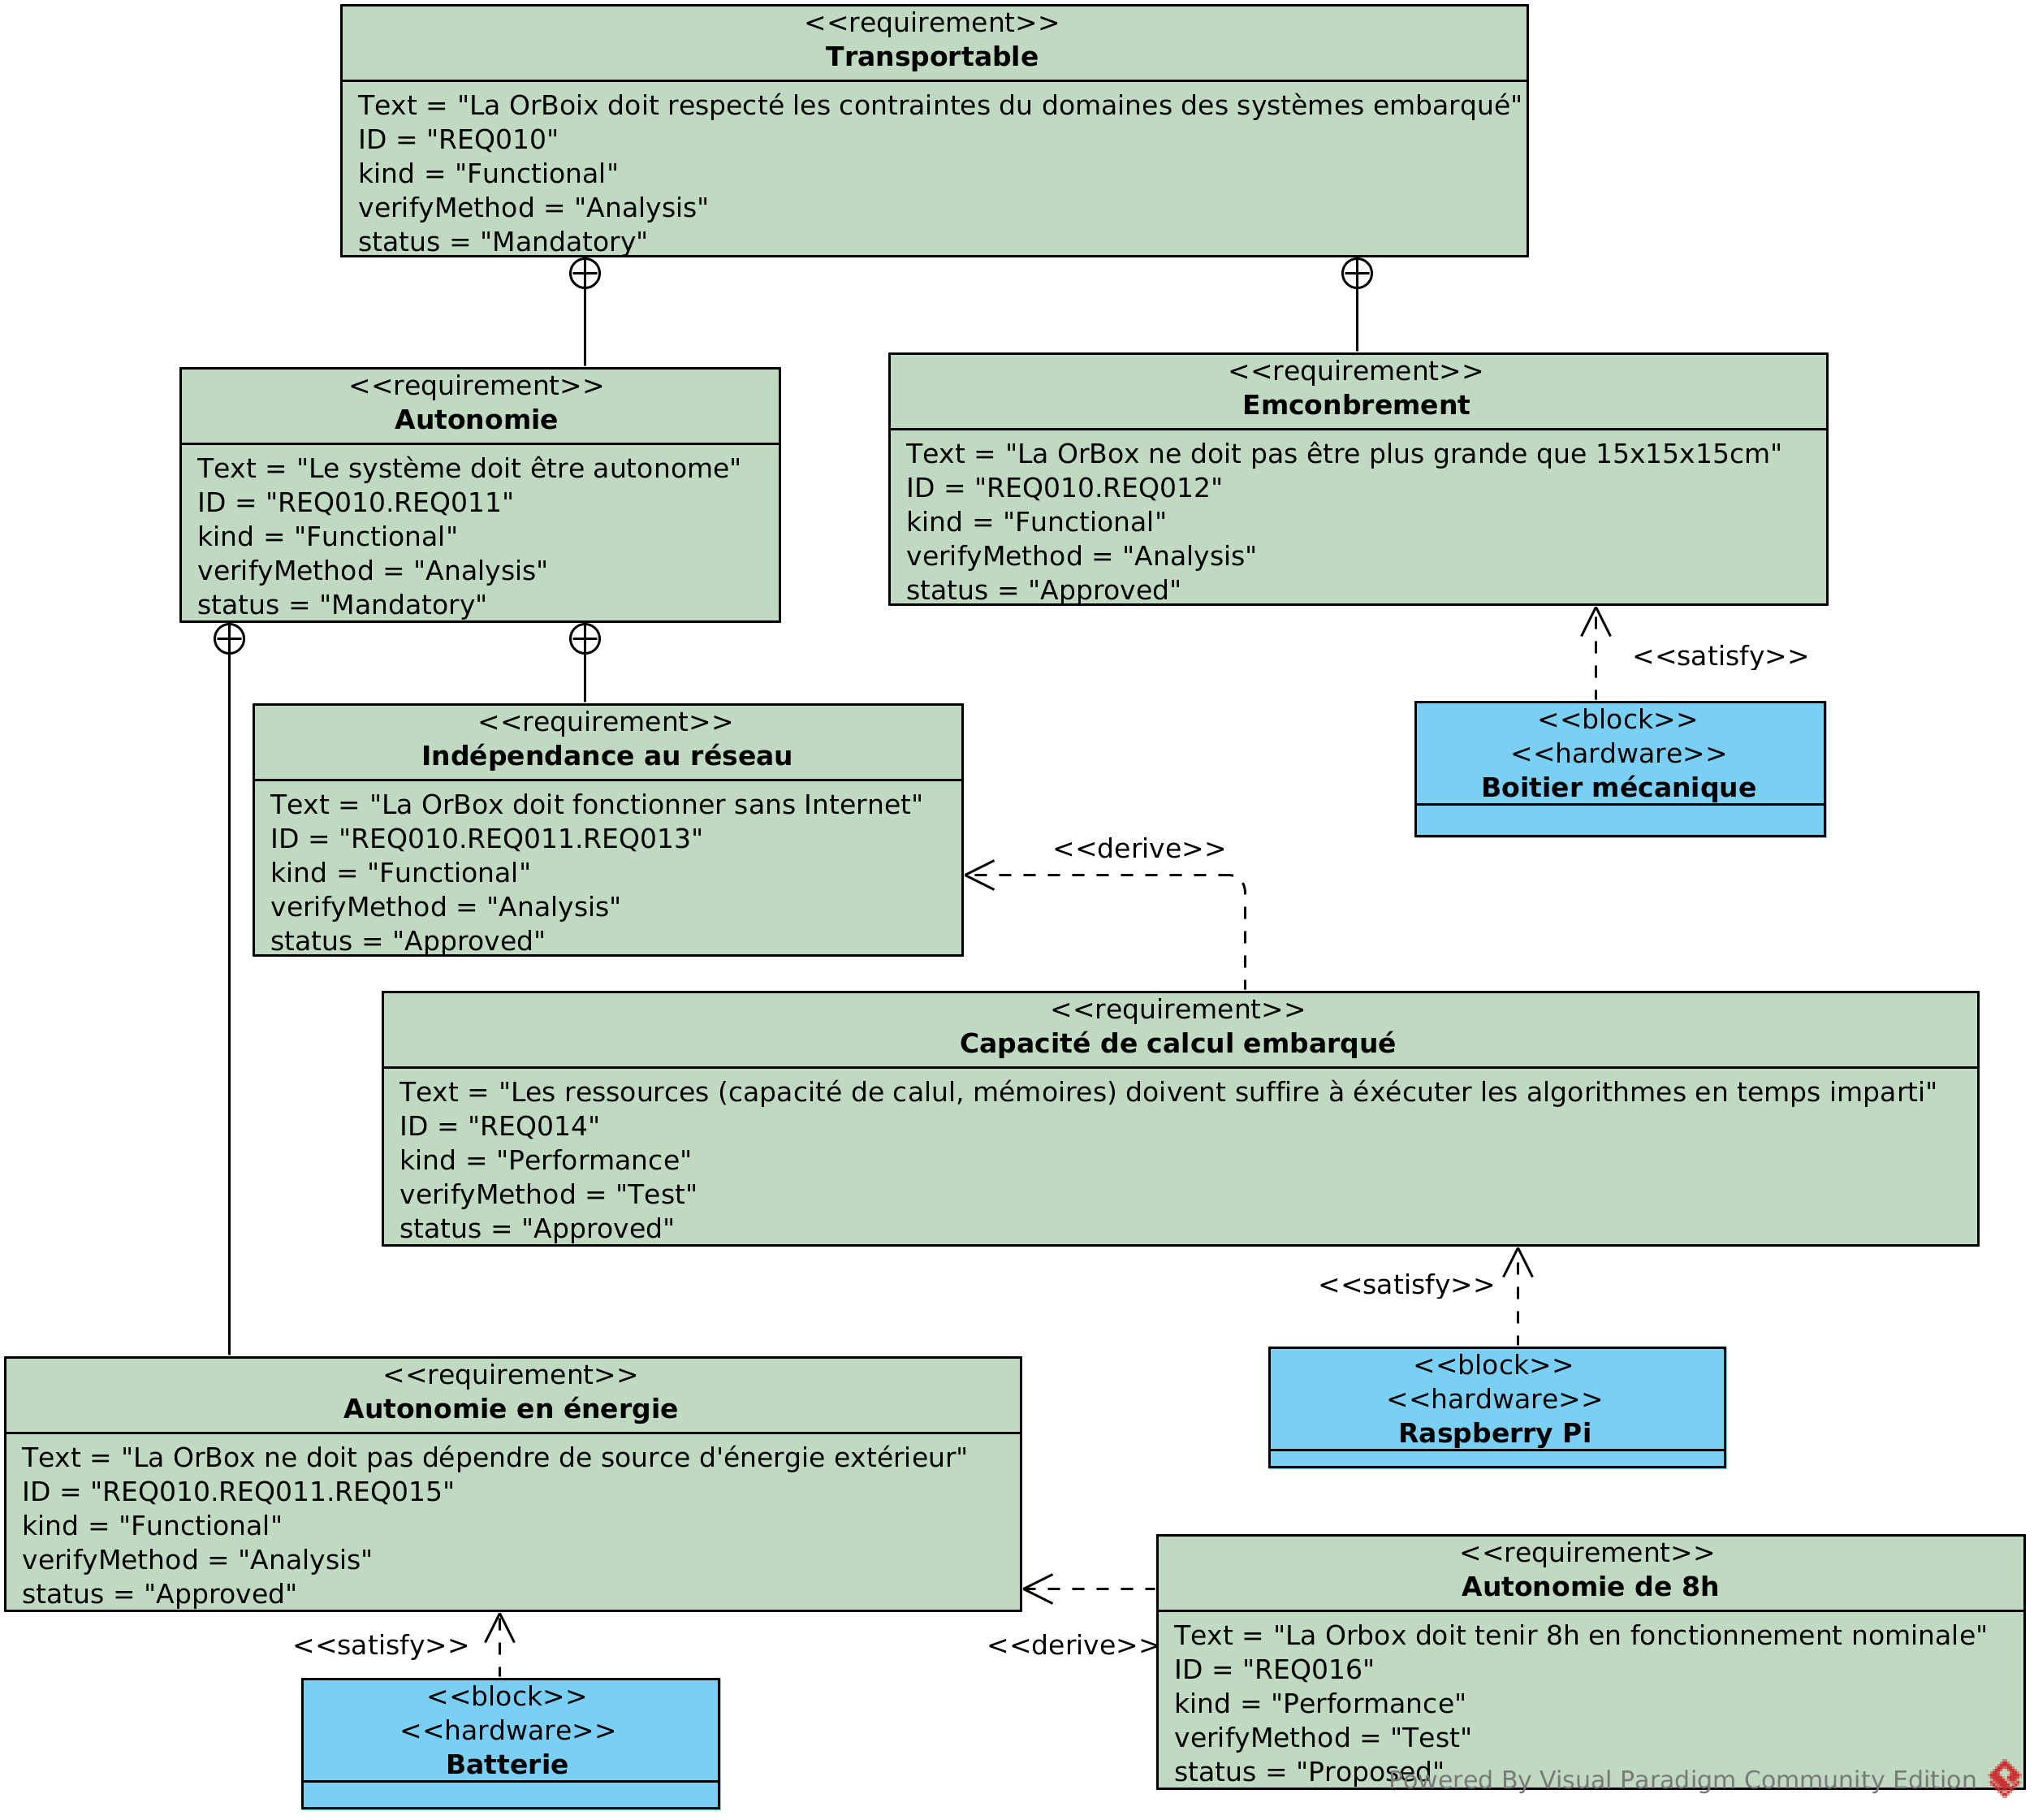
\includegraphics[scale=0.75]{img/SysML_Embedded_RD.png}
    \caption{Diagramme des exigences relatives aux systèmes embarqués}
    \label{RDEmbedded}
\end{figure}
		
\begin{figure}[H]
    \centering
    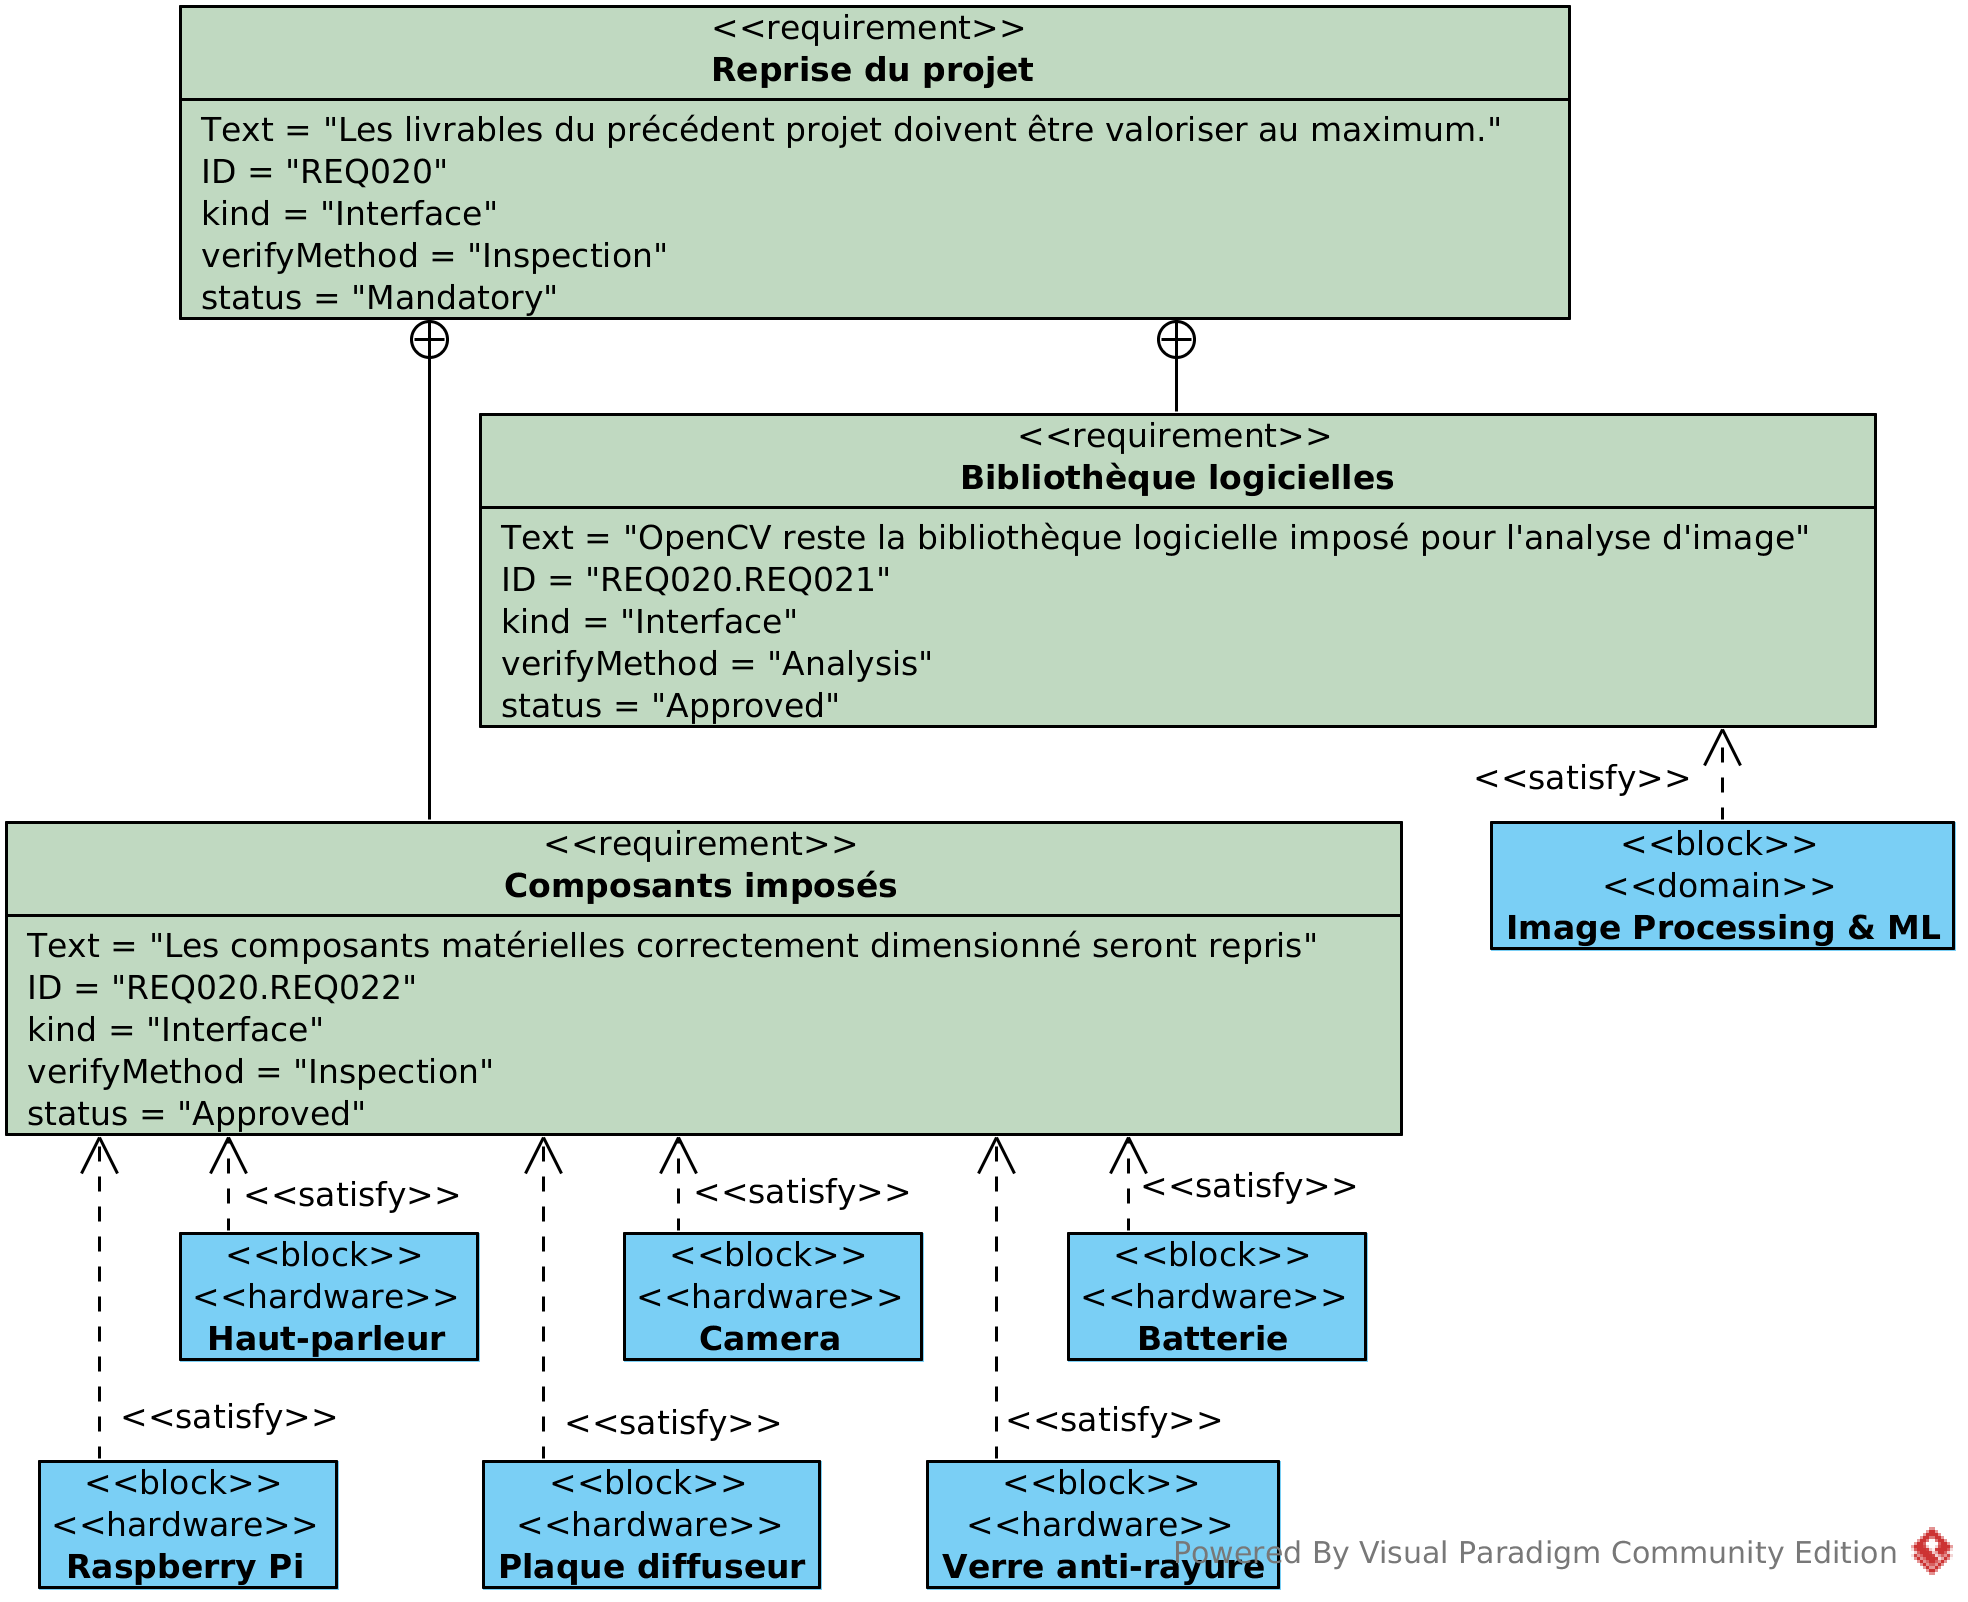
\includegraphics[scale=0.75]{img/SysML_Project_RD.png}
    \caption{Diagramme des exigences relatives à la reprise de projet}
    \label{RDProject}
\end{figure}


\section{Description des interfaces externes du logiciel}

		\subsection{Interfaces matériel/logiciel}

Pour avoir la liste des interfaces matérielles à piloter se référer à la figure~\ref{TopBDD} (p.\pageref{TopBDD}) elles y sont modélisées sous la forme de \emph{flow ports}.
Une description plus détaillée de chacune est faite dans les descriptions des fonctionnalités, notamment la section~\ref{sub:DefRPi} (p.\pageref{sub:DefRPi}).

	\subsection{Interfaces homme/machine}
	
Le système dans son ensemble est dédié à l'interface homme/machine, mais ils existent deux blocs logiciels dédier à deux aspects d'interfaçage :
\begin{itemize}
    \item Le bloc "IHM local" (cf section~\ref{sub:DefIHM} p.\pageref{sub:DefIHM}).
    \item Le bloc "Interface d'administration" (cf section~\ref{sub:DefAdmin} p.\pageref{sub:DefAdmin}).
\end{itemize}

	\subsection{Interfaces logiciel/logiciel}

Deux stratégies ont été employées :
\begin{itemize}
    \item La première consiste à l'utilisation d'une API REST afin d'accéder à des ressources logicielles communes --- cette approche est modélisée sur la figure~\ref{TopBDD} (p.\pageref{TopBDD}) par la relation d'utilisation "Interroge".
    Le détail des messages circulant est donné dans l'annexe \ref{annexe_api} (p. \pageref{annexe_api}).
    La figure~\ref{predictSD} (p.\pageref{predictSD}) montre l'utilisation de cette API pour un cas d'utilisation.
    \item La deuxième consiste à appeler des programmes dans des processus différents --- cette approche est modélisée sur la figure~\ref{TopBDD} (p.\pageref{TopBDD}) par la relation d'utilisation "Utilise".
    L'intérêt est d'avoir des programmes écrits en C++ (avec OpenCV) pour la partie Image Processing et Machine Learning qui soit performant, et de l'autre utiliser une technologie permettant de développer rapidement une application Web frontend (pour mobile ou desktop) et backend (avec Node.js ou Scalatra).
\end{itemize}

	
    \section{Architecture générale du système}
\label{sec:archi}

La figure \ref{TopBDD} ci-dessous montre l'architecture matérielle et logicielle du système global, elle suit le formalisme SysML.
Une description détaillée des composants est fournie dans les sous-sections ci-dessous.

\begin{figure}[H]
	\centerline{
		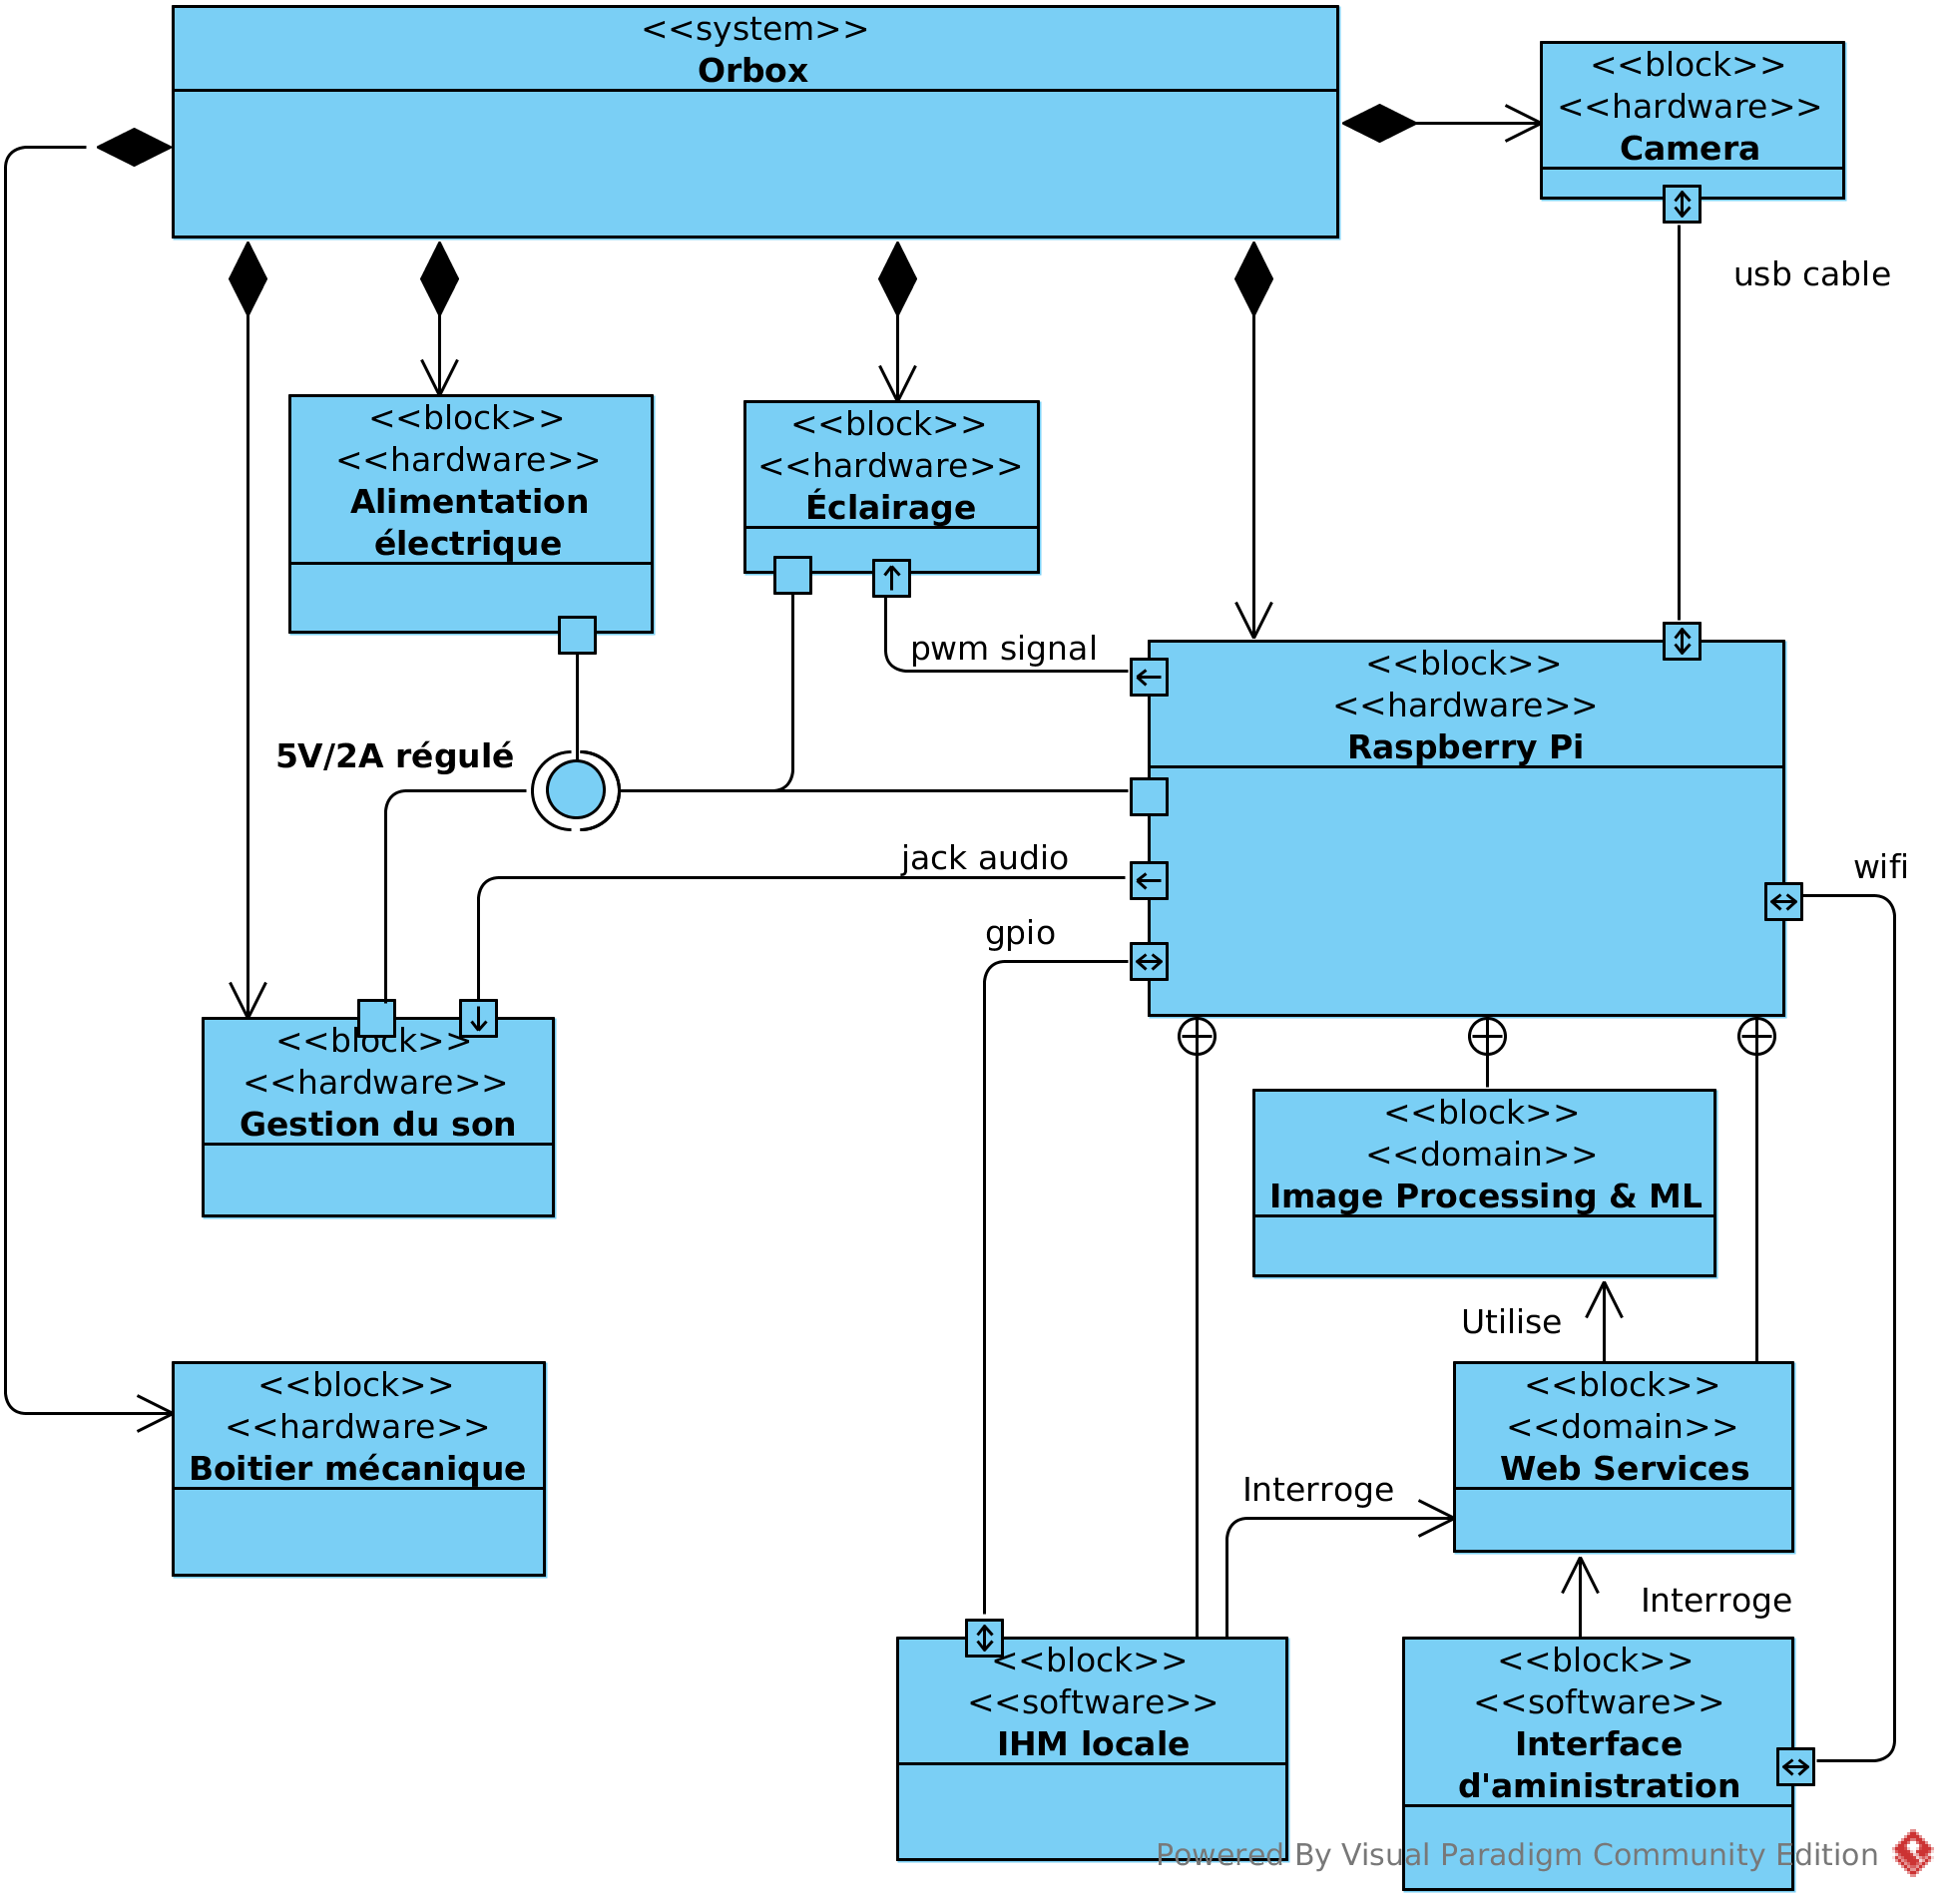
\includegraphics[scale=0.75]{img/SysML_Top_BDD.png}
	}
	\caption{Top level Block Definition Diagram}
	\label{TopBDD}
\end{figure}
    
    \section{Description des fonctionnalités}
\label{sec:fonctions}
%Il s'agit de l'expression des besoins fonctionnels. Cette partie a donc comme objectif de décrire l'ensemble des fonctionnalités du système en précisant avec quels composants de la partie~\ref{sec:archi} elles interagissent. Des diagrammes de cas d'utilisation plus détaillés que ceux présentés en~\ref{sec:foncgales}, ainsi que l'arbre hiérarchique des fonctionnalités pourront être fournis ici pour donner une vision plus globale. En outre, chaque fonctionnalité sera décrite précisément (cf.ci-dessous). Là encore, il s'agit d'une pré-analyse indispensable à l'évaluation de la complexité de votre projet et à la planification de sa réalisation.

    \subsection{Définition du bloc Alimentation électrique}
\label{sub:DefAlim}

Ce bloc a pour rôle de fournir l'énergie de manière suffisante et appropriée aux composants électroniques de la Or-Box.
Il doit répondre à la contrainte d'autonomie du système.
Le bloc \emph{Alimentation électrique} est composé de quatre éléments --- visibles sur la figure \ref{AlimBDD}.

\begin{figure}[H]
	\centerline{
		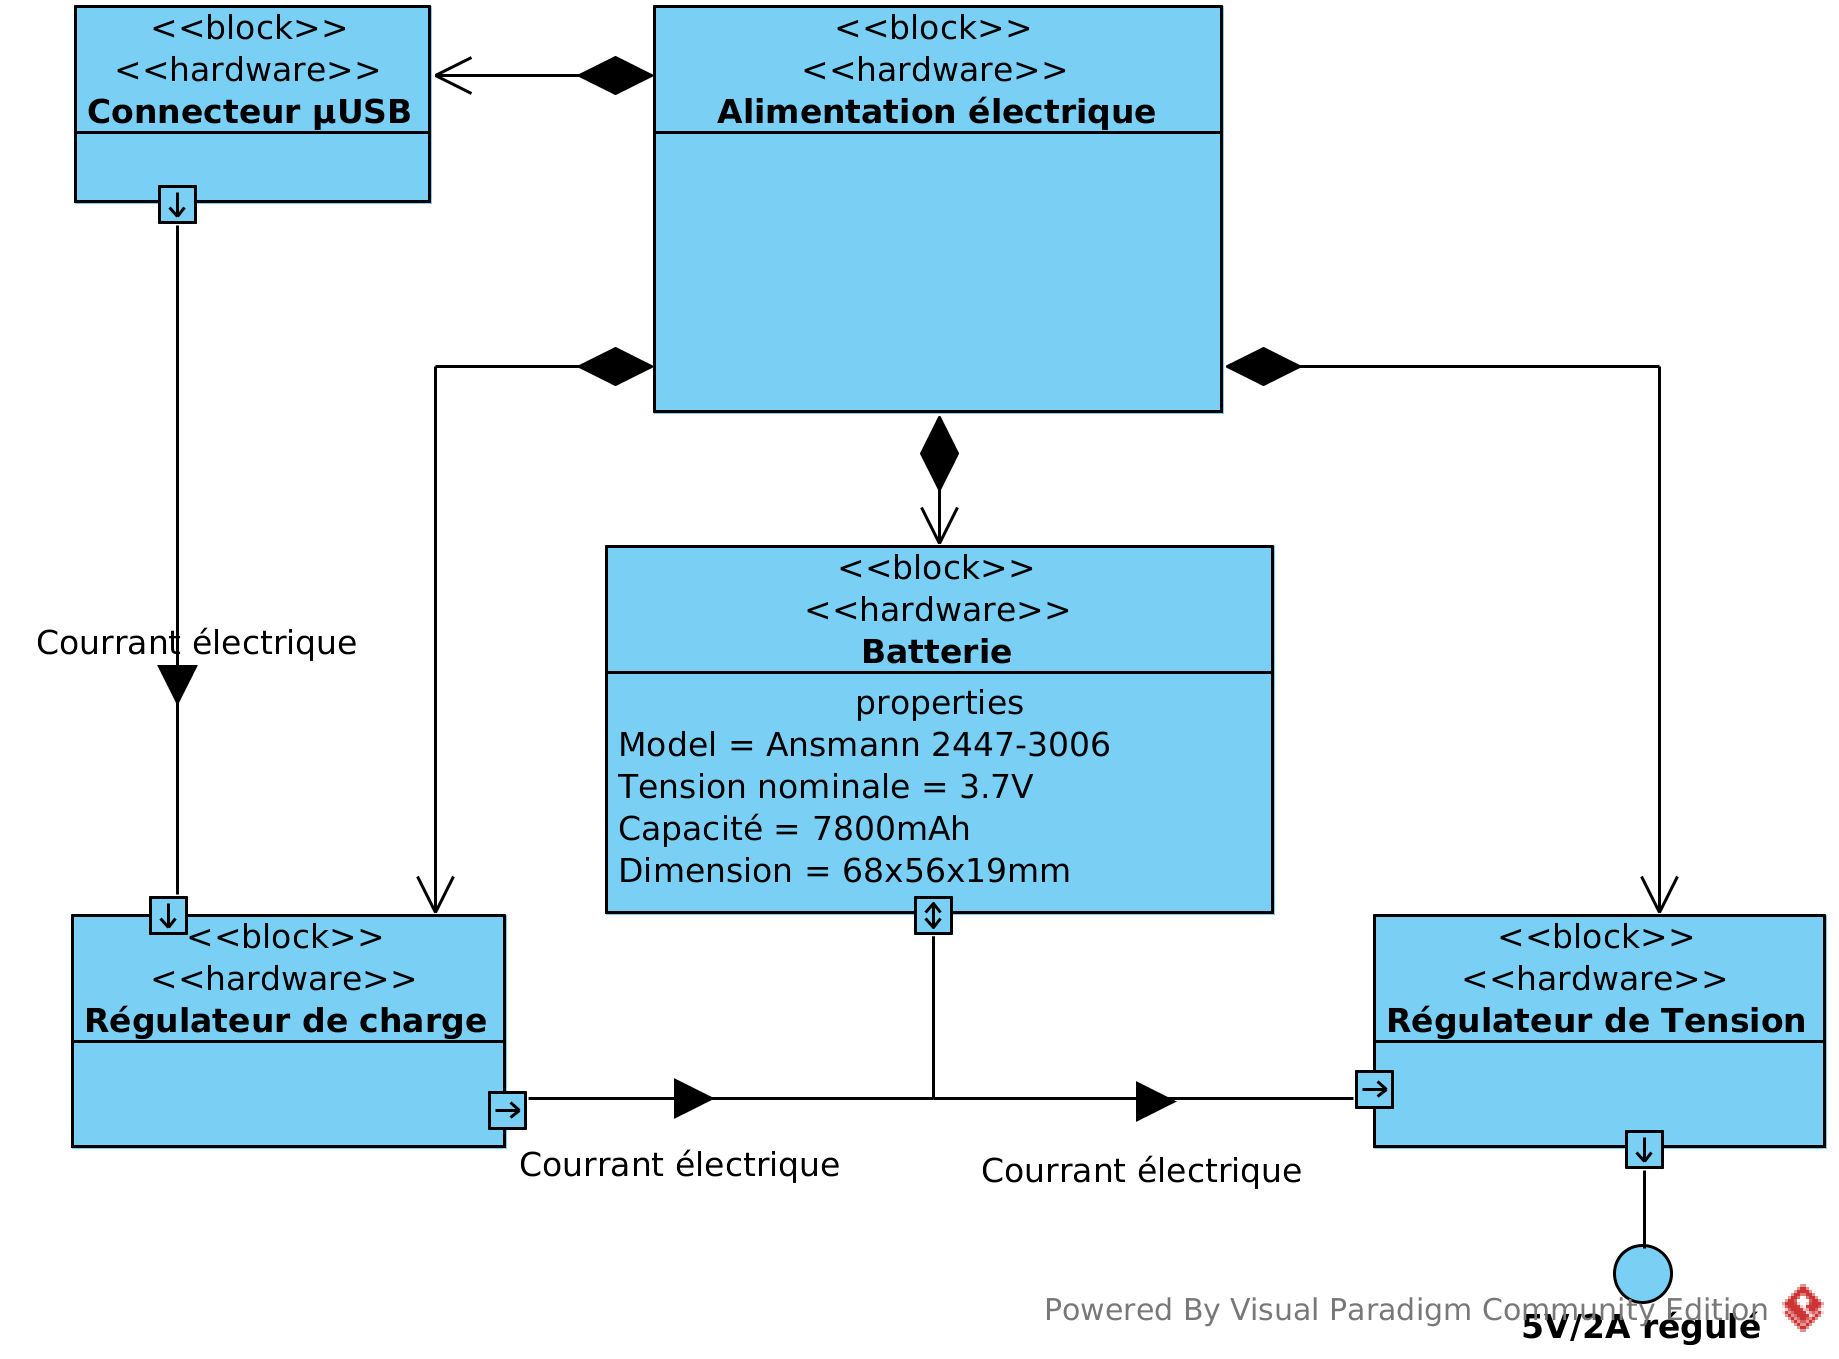
\includegraphics[scale=0.75]{img/SysML_Alim_BDD.png}
	}
	\caption{Alimentation électrique --- Block Definition Diagram}
	\label{AlimBDD}
\end{figure}

\begin{labeling}[~--]{Connecteur micro-USB}
	\item [Batterie]
	Elle permet de stocker l'énergie sous forme électrochimique.
	Il s'agit d'une batterie de technologie Lithium-Ion.
	\\ \emph{Bloc imposé --- héritage de la version précédente.}
	\item [Régulateur de charge]
	Il doit adapter l'énergie électrique fournie par un chargeur USB mural pour charger la batterie de manière sûre.
	Il devra aussi fournir une indication sur l'état de la charge.
	\item [Régulateur de tension]
	Il doit adapter l'énergie électrique fournie par la batterie aux composants électroniques de la Or-Box.
	Le composant le plus critique est la Raspberry Pi, elle doit être alimentée en 5V --- cette tension d'alimentation servira de critère dans la sélection des autres composants afin de ne pas multiplier les régulateurs de tension.
	\item [Connecteur micro-USB]
	Il doit permettre la connexion d'un chargeur mural.
	La connectique USB micro a été choisie, car il s'agit de la plus répandue aujourd'hui.
\end{labeling}


% subsection DefAlim (end)

    \subsection{Définition du bloc Boitier mécanique}
\label{sub:DefMeca}

Ce bloc a pour rôle de donner une unité matérielle à l'ensemble des composants composant la Or-Box --- c'est-à-dire les blocs identifiés avec le stéréotype \emph{<<hardware>>} sur les diagrammes SysML.
Le bloc \emph{Boitier mécanique} est composé de trois éléments --- visibles sur la figure \ref{MecaBDD}.


\begin{figure}[H]
	\centerline{
		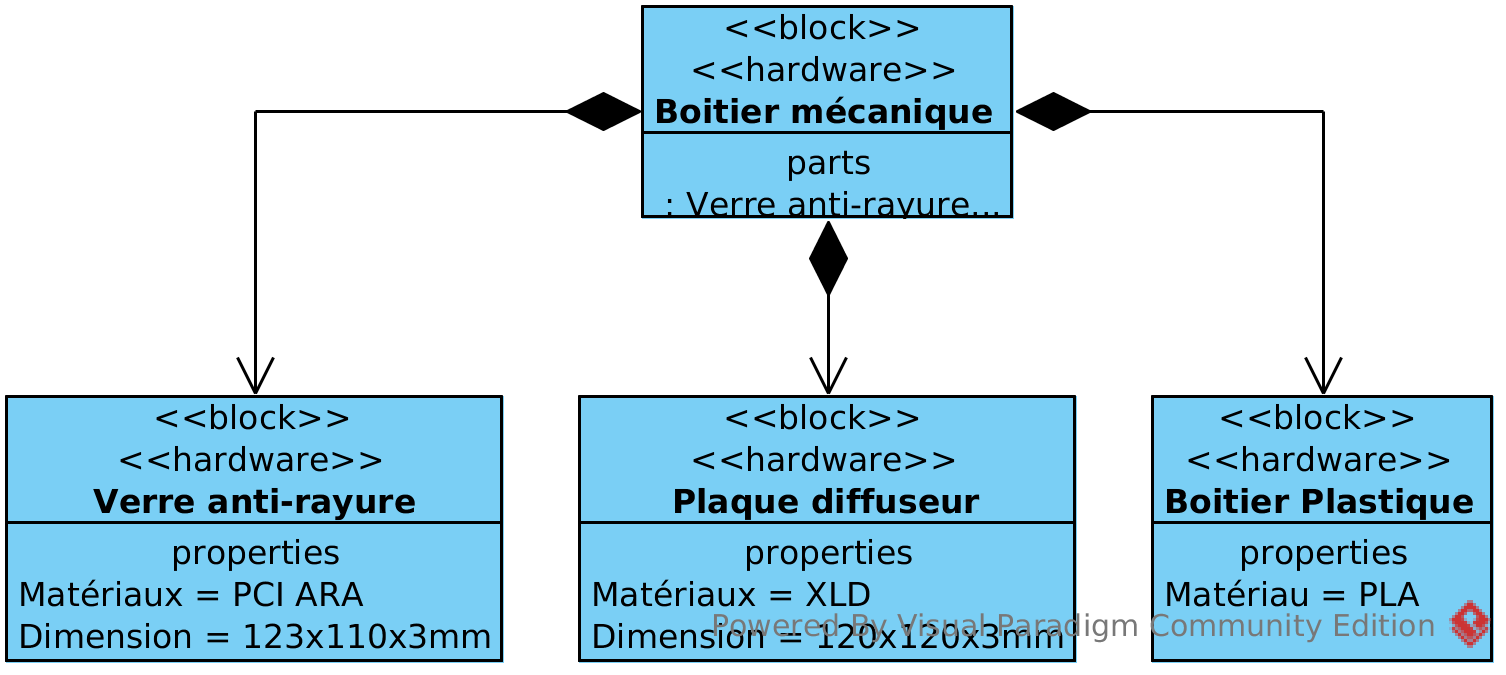
\includegraphics[scale=0.75]{img/SysML_Meca_BDD.png}
	}
	\caption{Boitier mécanique --- Block Definition Diagram}
	\label{MecaBDD}
\end{figure}

\begin{labeling}[~--]{Verre anti-rayure}
	\item [Boitier plastique]
	Il doit être fabricable avec les moyens matériels disponibles à Polytech, principalement des imprimantes 3D \emph{Ultimaker II}.
	Cette contrainte impose donc une taille maximum des pièces de 230x225x205 mm.
	Avec l'expérience de l'an passé, une contrainte de maintenance a été ajoutée : le boitier doit permettre un désassemblage aisé et non destructif des autres éléments mécaniques. 	
	\item [Verre anti-rayure]
	Il constitue la surface sur laquelle seront posés les objets à identifier.
	Il est translucide et fait d'un matériau anti-rayure pour en préserver la qualité optique à travers le temps.
	Il a été montré par l'expérimentation que la distance entre l'objectif de la caméra et le verre devait être d'un minimum de 3 cm afin d'avoir une visibilité de l'intégralité de la surface de reconnaissance.
	\\ \emph{Bloc imposé --- héritage de la version précédente.}
	\item [Plaque diffuseur]
	Elle permet de diffuser la lumière générée par les LED situées en dessous afin d'offrir un éclairage uniforme sur toute la surface.
	Afin d'offrir les meilleures performances, une distance minimum de 4 cm doit être maintenue avec la source lumineuse.
	\\ \emph{Bloc imposé --- héritage de la version précédente.}	
	
\end{labeling}

% subsection DefMeca (end)

\subsection{Définition du bloc Gestion du son}
\label{sub:DefSon}

Ce bloc a pour rôle de transformer et d'adapter le signal électrique en signal sonore.
Deux composants ont été identifiés (visible sur la Figure \ref{SonIBD}) ; l'amplificateur audio, qui prend le signal électrique fourni par le DAC du Raspberry Pi et l'amplifie pour le haut-parleur de la Or-Box (\emph{Bloc imposé --- héritage de la version précédente.}). 

\begin{figure}[H]
	\centerline{
		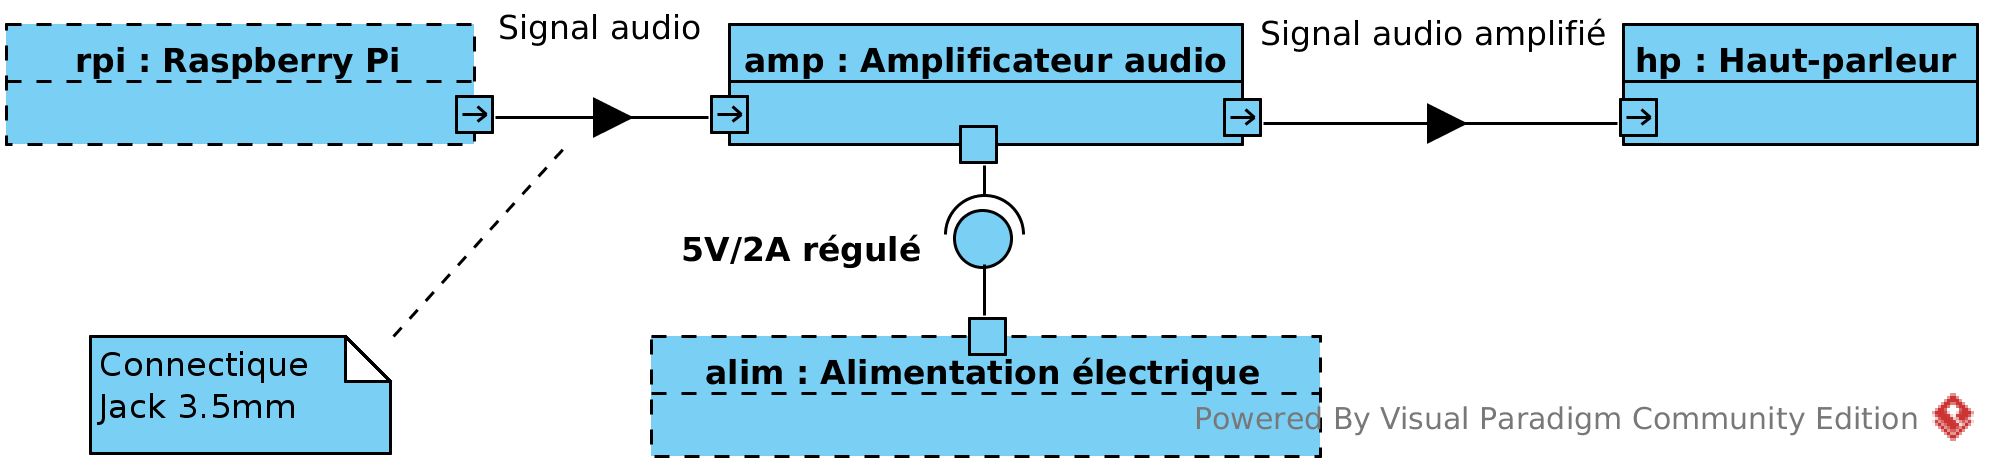
\includegraphics[scale=0.75]{img/SysML_Son_IBD.png}
	}
	\caption{Gestion du son --- Internal Block Diagram}
	\label{SonIBD}
\end{figure}


% subsection DefSon (end)
\subsection{Définition du bloc Éclairage}
\label{sub:DefEclairage}

L'éclairage permet d'avoir des clichés des objets posés sur la vitre malgré le contre-jour créé par la lumière ambiante.
Afin de limiter la complexité du routage du PCB, on utilisera un Driver de LED pour piloter les LED.

\begin{figure}[H]
	\centerline{
		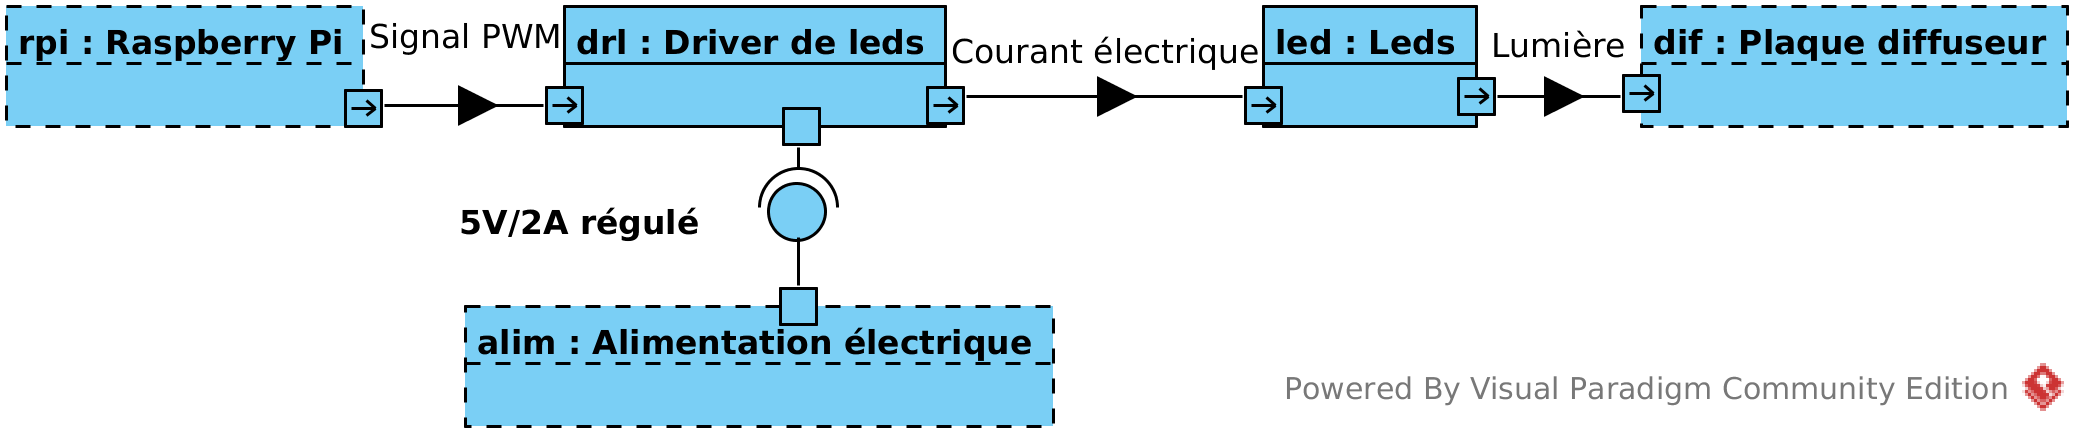
\includegraphics[scale=0.75]{img/SysML_Lum_IBD.png}
	}
	\caption{Éclairage --- Internal Block Diagram}
	\label{LumIBD}
\end{figure}


% subsection DefEclairage (end)

\subsection{Définition du bloc Caméra}
\label{sub:DefCam}
\emph{Block imposé --- héritage de la version précédente.}

Le bloc caméra est un COTS.
Il s'agit d'une caméra USB de chez \emph{ELP CCTV} --- ELP-USBFHD01M-L170.
Elle est équipée d'un objectif de 170 \degree d'angle de vue.
Elle fournit un flux vidéo en 1920x1080 MJPEG@30fps.


Elle est compatible avec la bibliothèque \emph{V4L}, la librairie utilisée par OpenCV pour la capture de flux vidéo.
L'expérience de l'an passé nous a montré que le temps entre la demande d'ouverture du flux vidéo et la première image disponible était supérieur à 2 secondes --- notre principale contrainte de performance.
Ceci nous oblige à allumer la caméra en permanence, réduisant drastiquement l'autonomie du système.

% subsection DefCam (end)
\subsection{Définition du bloc Raspberry Pi}
\label{sub:DefRPi}
\emph{Bloc imposé --- héritage de la version précédente.}

Le Raspberry Pi est un ordinateur mono carte prévu pour les applications de développement embarqué.
Il n'est cependant pas prévu pour une utilisation en production.
En effet, il fonctionne sur carte SD, trop sensible aux vibrations, l'utilisation d'une mémoire eMMC est préférable pour les systèmes embarqués.
Aussi il embarque un nombre très important de périphériques, certains ne seront pas exploités dans la Or-Box (par exemple la sortie HDMI de l'écran), mais ils peuvent parfois se révéler très utiles lors du développement.
Le projet se limitant au cadre d'un prototype, il a donc été décidé de continuer le développement sur cette carte avec l'OS Raspian Lite. 


Le Raspberry Pi utilisera les entrées/sorties suivantes :
\begin{description}
    \item [Un port USB 2.0] Afin de capturer le flux vidéo de la Webcam.
    Le port est bidirectionnel, car il est nécessaire d'envoyer des paramètres de configurations (autofocus OFF, résolution, framerate\ldots) lors de démarrage de la caméra.
    \item [Le Wi-Fi.] Soit par l'intermédiaire d'un dongle USB dans le cas d'une Raspberry Pi 2, soit en utilisant le chip intégré de la Raspberry Pi 3.
    Il sera utilisé pour communiquer avec un terminal distant (Smartphone ou Desktop) à travers un port HTTPS.
    \item [Jack audio 3.5 mm.] Afin de profiter du DAC audio de la Raspberry Pi, la solution la moins intrusive est d'utiliser cette connectique.
    \item [Pin PWM.] Cette sortie sert à piloter l'éclairage.
    En modulant la largeur d'impulsion entre 0~et~1 on peut éteindre l'éclairage, éclairer à la luminosité maximum ou profiter de la plage entre ces deux extremums.
    \item [Pins GPIO.] Deux pins seront utilisés, un configuré en entrée, le deuxième en sortie.
    Le premier servira à lire l'état du bouton-poussoir, deux scénarios seront enclenchés suivant la durée de l'appui.
    L'appuie long pour l'extinction du Raspberry pi, le court pour la capture d'images, l'analyse et la lecture du message audio approprié.
    Le deuxième pin servira à piloter une LED afin de communiquer sur l'état de la Raspberry Pi.
    La LED sera fixe pendant la période de boot, clignotante quand tous les composants logiciels ont correctement démarré et la Or-Box prête, et éteinte quand la Raspberry Pi est éteinte et l'alimentation prête à être coupé.
\end{description}
% subsection DefRPi (end)

\subsection{Définition du bloc Interface d'administration}
\label{sub:DefAdmin}

Ce composant logiciel est le seul à ne pas être exécuté sur la Raspberry Pi.
Il pourra s'agir soit d'une application pour smartphone, soit d'une application dans le navigateur.
La communication avec la Or-Box est faite via le Wi-Fi.
Les différentes actions réalisables sont implémentées sous la forme de web services REST.
% subsection DefAdmin (end)

\subsection{Défintion du bloc IHM Locale}
\label{sub:DefIHM}

Ce composant logiciel a pour but d'orchestrer les scénarios de la Or-Box quand elle utilisé de manière autonome.
Afin de ne pas dupliquer certaines fonctionnalités le déroulement des scénarios s'appuiera aussi sur l'utilisation des web services implémentés --- ils ne passeront cependant pas sur le Wi-Fi, mais resteront sur la boucle locale.
Ce bloc logiciel sera implémenté soit en Shell, Python ou C++.

Le premier scénario --- et le plus important --- est la prédiction de la classe à laquelle les différents objets présents sur la vitre appartiennent ; ce scénario est déclenché par un appui court sur le bouton-poussoir en façade de la Or-Box.
La figure \ref{predictSD} montre les différents appels aux web services faits par le bloc IHM locale pour ce scénario.

\begin{figure}[H]
    \centering
    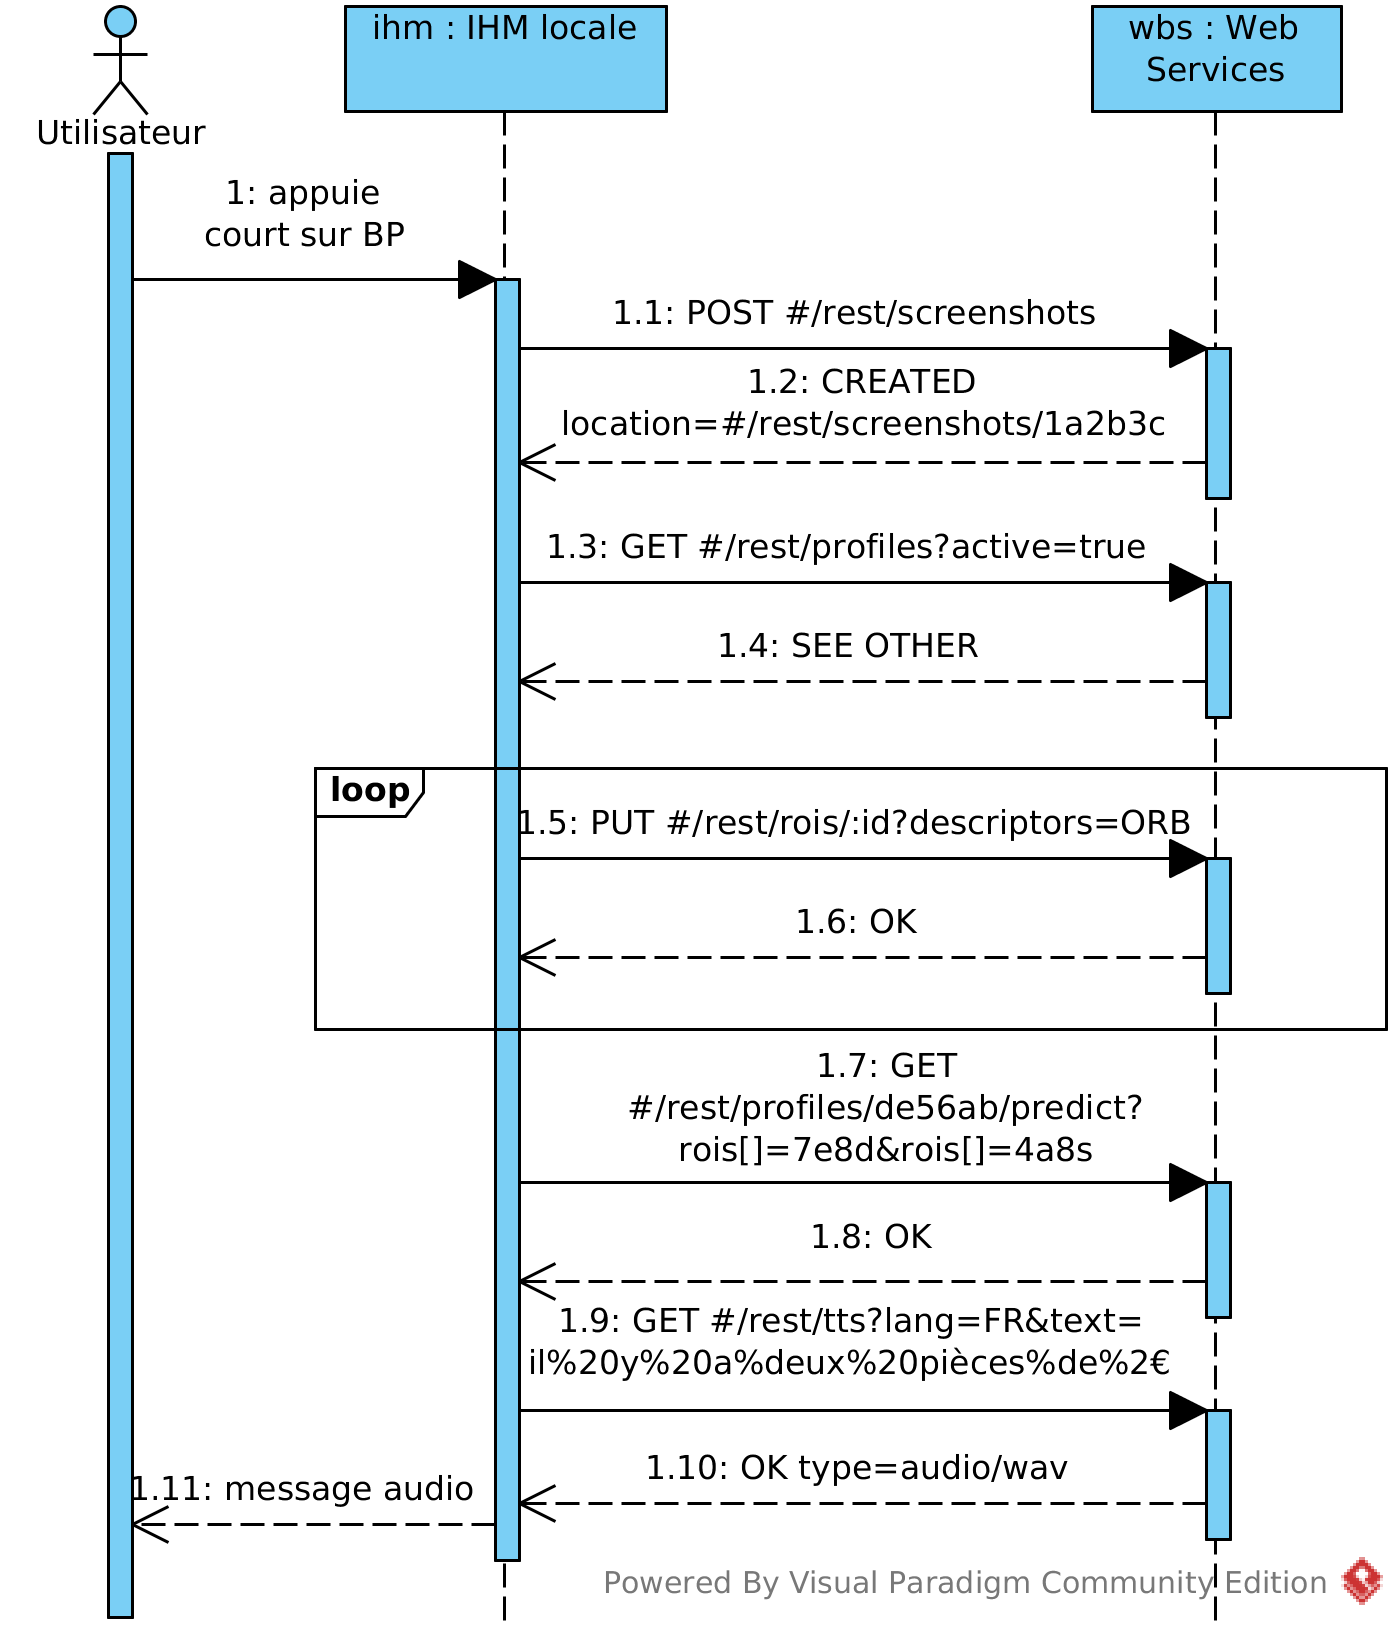
\includegraphics[scale=0.75]{img/SysML_Predict_SD.png}
    \caption{Diagramme de séquence pour le scénario de prédiction}
    \label{predictSD}
\end{figure}

Le deuxième scénario est l'extinction de la Raspberry Pi par un appui long sur le bouton-poussoir.


% subsection DefIHM (end)

\subsection{Définition du bloc Web Services}
\label{sub:DefWebServices}

Des ressources devront être accédées par l'interface distante d'administration et par l'IHM locale, afin d'harmoniser l'accès à ces ressources des Web Services seront créer.
L'architecture de ces services essaie de respecter l'architecture REST ; notamment le principe de HATEOAS.

L'API de ces Web Services est décrite ressource par ressource dans les annexes.
Toutes les données transmises sont du type "application/hal+json" sauf si autrement spécifié.

% subsection DefWebServices (end)

\subsection{Définition du bloc Image Processing \& Machine Learning}
\label{sub:DefCVML}

Ce bloc logiciel contient le coeur de métier de l'application.


\begin{figure}[H]
    \centering
    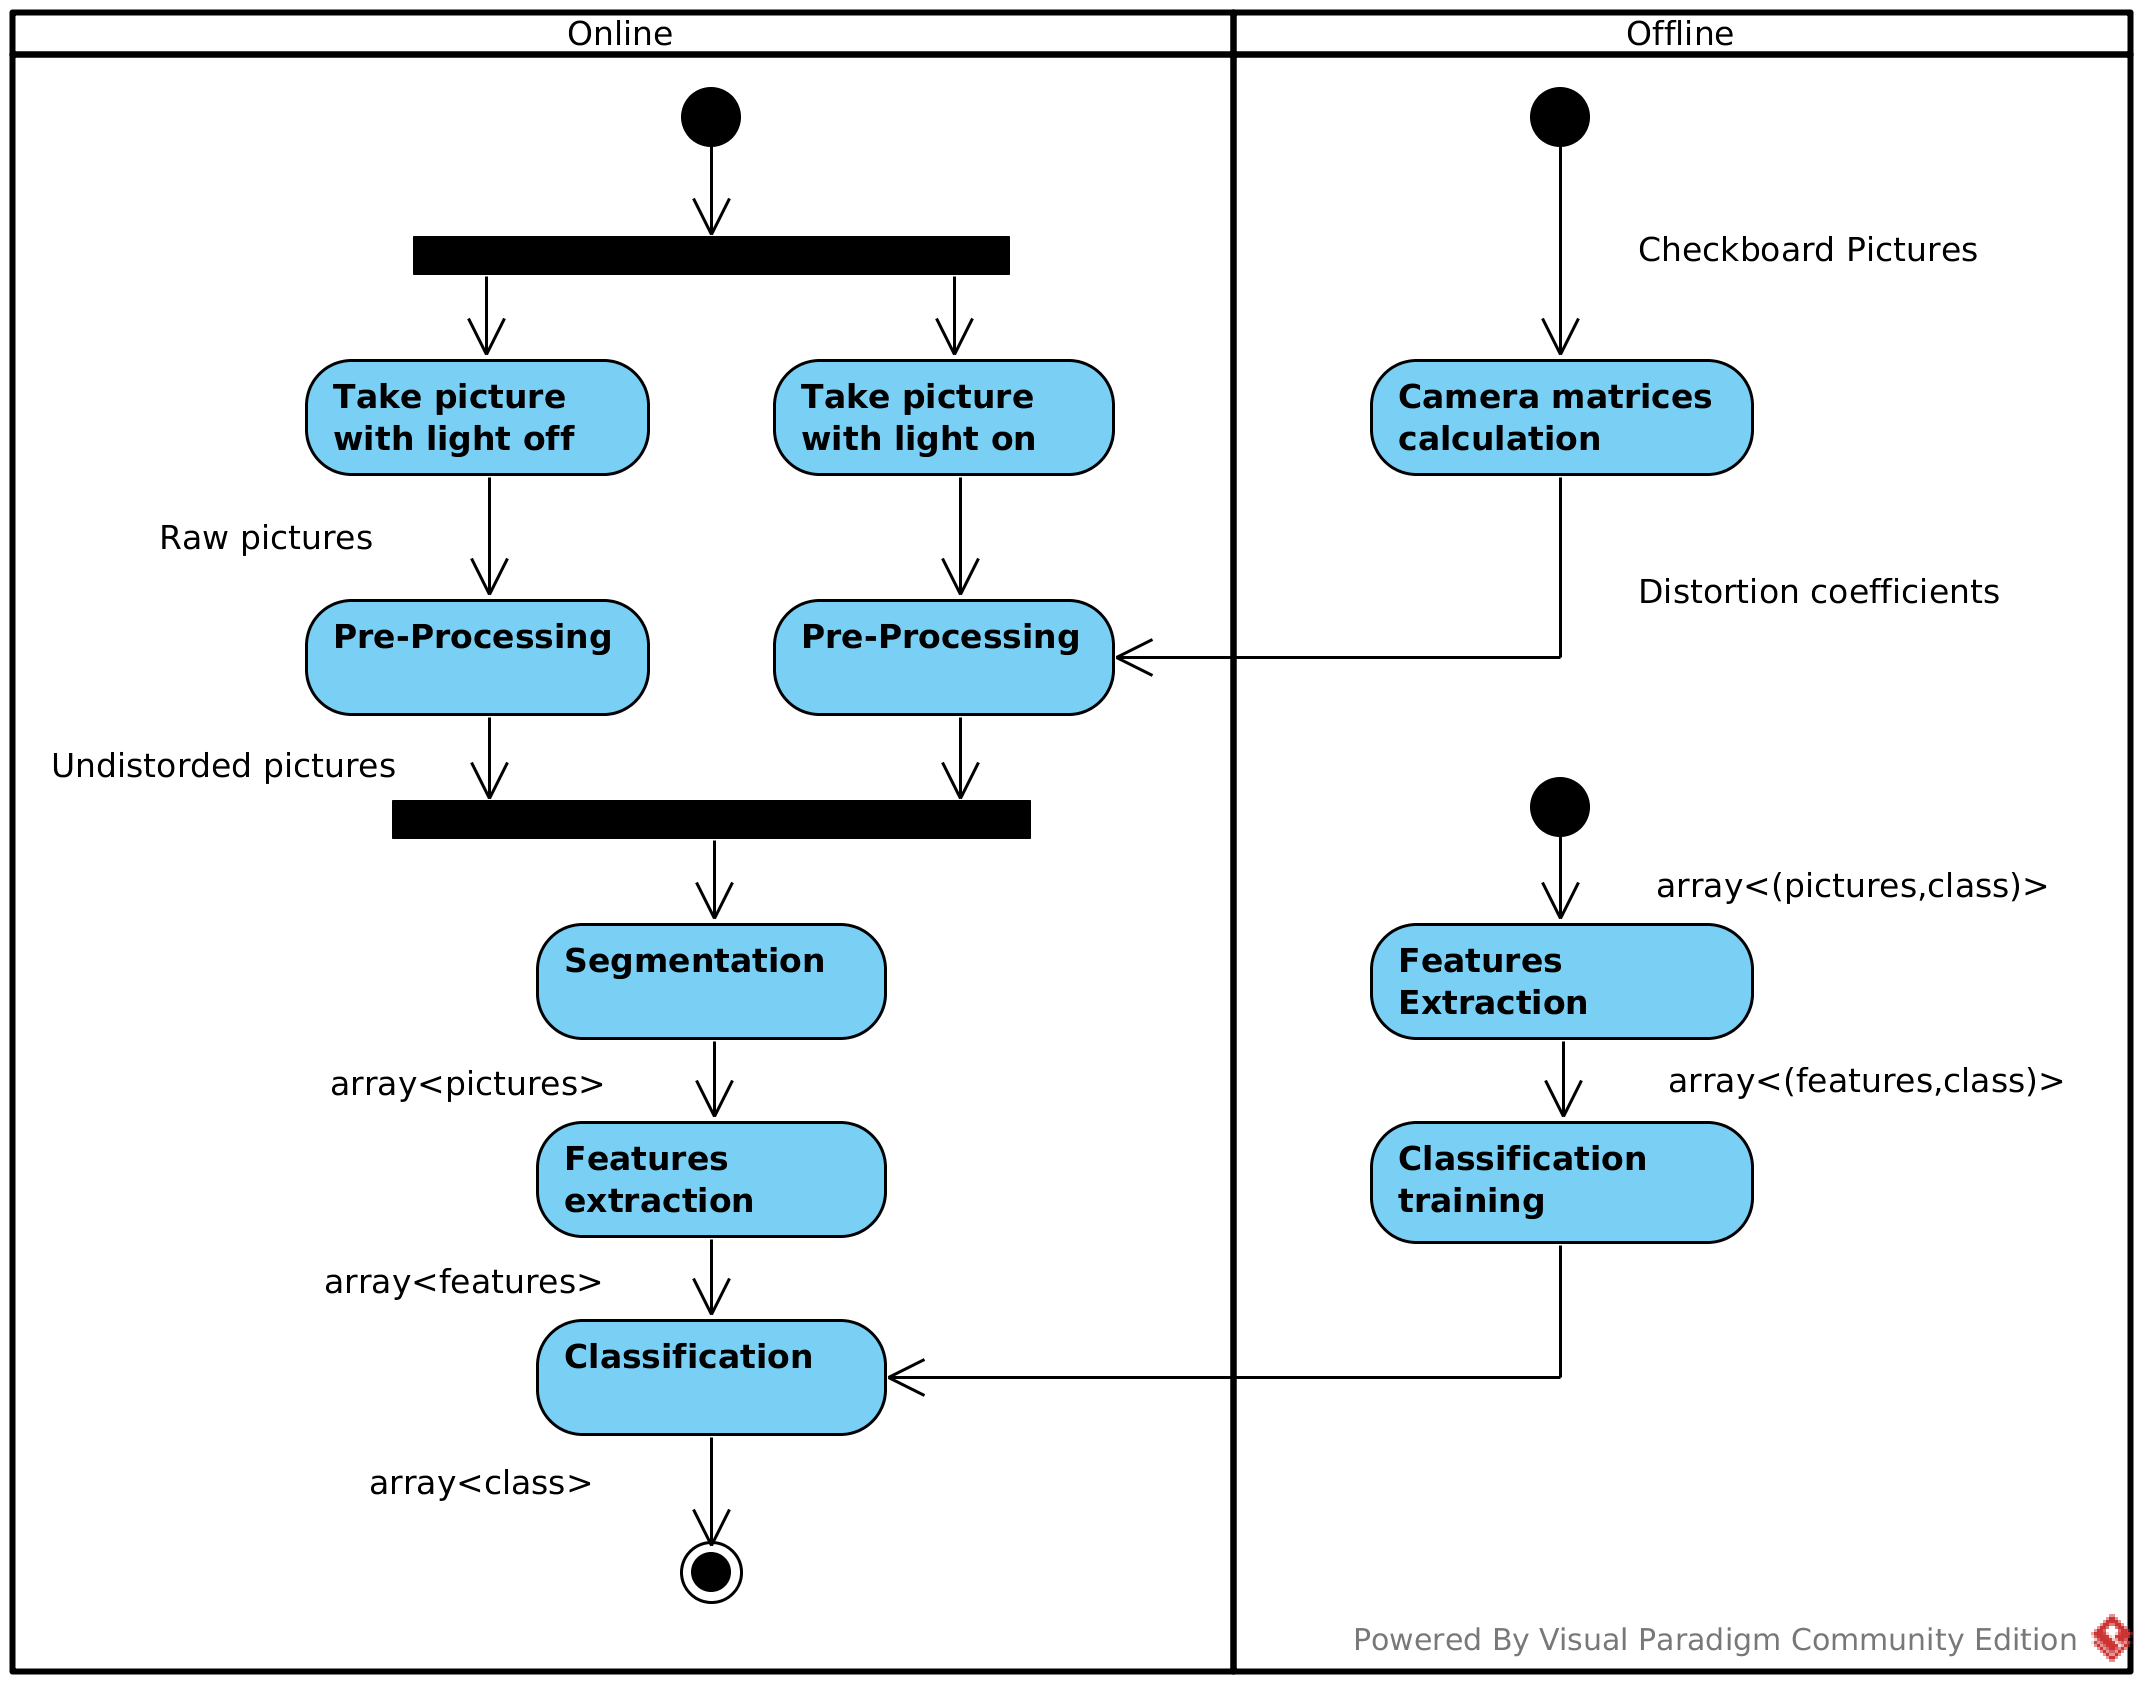
\includegraphics[scale=0.75]{img/SysML_CVML_AD.png}
    \caption{Diagramme d'activité --- Image processing \& Machine Learning}
    \label{CVMLAD}
\end{figure}

\section{Conditions de fonctionnement}

	\subsection{Performances}
	
Les contraintes de performances sont indiquées dans la section \ref{Contraintes} à travers les exigences typées \emph{"performances"} dans les trois diagrammes d'exigences.

	\subsection{Capacités}
	
Dans son fonctionnement nominal, la Or-Box n'aura pas de problème de charge de travail.
Un seul utilisateur à la fois interagira avec le système, que se soit pour avoir des informations sur l'objet ou lors de l'administration. Une étude plus approfondie sur le sujet doit être menée si la Or-Box venait à être industrialisée --- hors des objectifs établies (voir la section~\ref{sec:objectifs} p.\pageref{sec:objectifs}).

    \subsection{Contrôlabilité}

On effectuera la journalisation des algorithmes du bloc \emph{Image Processing \& Machine Learning} pour juger des critères de performances \footnote{voir section \ref{sub:DefCVML}}.

    \subsection{Sécurité}

La sécurité logicielle de la Or-Box ne fait pas partie des préoccupations de ce projet, car il s'agit d'une contrainte liée à la phase d'industrialisation du produit (voir la section~\ref{sec:objectifs} p.\pageref{sec:objectifs}).